\synctex=1
\documentclass[12pt,a4paper,oneside]{article}

\usepackage[spanish]{babel}

\usepackage{fancyhdr}
\usepackage{geometry}
\usepackage{graphicx}
\usepackage{wrapfig}
\usepackage{lastpage}
\usepackage[hidelinks]{hyperref}
\usepackage{authblk}
\usepackage{bookmark}

\usepackage[utf8]{inputenc} % Required for inputting international characters
\usepackage[T1]{fontenc} % Output font encoding for international characters
\usepackage{mathpazo} % Palatino font

\makeatletter
\newcommand{\subtitledoc}[1]{\newcommand{\@subtitledoc}{#1}}
\newcommand{\instituto}[1]{\newcommand{\@instituto}{#1}}
\newcommand{\carrera}[1]{\newcommand{\@carrera}{#1}}
\newcommand{\professor}[1]{\newcommand{\@professor}{#1}}
\newcommand{\catedraCaratula}[1]{\newcommand{\@catedraCaratula}{#1}}
\newcommand{\catedraHeader}[1]{\newcommand{\@catedraHeader}{#1}}
\newcommand{\curso}[1]{\newcommand{\@curso}{#1}}
\newcommand{\legajo}[1]{\newcommand{\@legajo}{#1}}
\newcommand{\footerauthor}[1]{\newcommand{\@footerauthor}{#1}}
\newcommand{\footerlegajo}[1]{\newcommand{\@footerlegajo}{#1}}

%Configuracion de hoja (margenes y tamaño)
\geometry{a4paper,margin=1in}
\setlength\headheight{28pt}

%formato de encabezado y pie para todas las paginas.
\fancyhead[L]{
    \begin{minipage}[b]{7.5mm}
        
\includegraphics[width=7mm]{Imagenes/logo-utn.png}
    \end{minipage}
    \begin{minipage}[b]{90mm}
        \textbf{Alumnos: }\@footerauthor \\
        \textbf{Legajos: }\@footerlegajo
    \end{minipage}
}
\fancyhead[R]{
    \textbf{Curso:} \@curso\\
    \textbf{Cátedra:} \@catedraHeader
}
\fancyfoot[L]{\@date}
\fancyfoot[C]{} %eliminar antiguo numero de pagina
\fancyfoot[R]{Página \thepage\ de \pageref{LastPage}}
\renewcommand{\headrulewidth}{0.5pt}
\renewcommand{\footrulewidth}{0.5pt}
\pagestyle{fancy}

\addto\captionsspanish{%
	\renewcommand{\contentsname}%
	{CONTENIDO}%
}

\renewcommand{\maketitle}{%
    \newpage
    \thispagestyle{empty}
    
    \begin{center}

    \textsc{\LARGE \@instituto}\\[0.5cm] 
    \textsc{\Large \@carrera}\\[1.5cm] 
    
\includegraphics[width=0.30\textwidth]{Imagenes/logo-utn.png} \par
    \vspace{1.5cm}
    
    \textsc{\large \@catedraCaratula }\\[0.5cm]
    
    {\huge\bfseries \@title}\\[0.4cm]
    \textsc{\Large \@subtitledoc}\\[0.5cm]
    

    \end{center}

    \vspace{2cm}

    {\noindent
    \begin{minipage}[t]{.2\textwidth}
        \raggedright
        \textbf{ALUMNOS} \par
        ~\\
        ~\\
        ~\\
        \textbf{CURSO} \par
        ~\\
        \textbf{DOCENTES} \par
        \end{minipage}%
     \begin{minipage}[t]{.05\textwidth}
        \raggedright
        \textbf{:} \par
        ~\\
        ~\\
        ~\\
        \textbf{:} \par
        ~\\
        \textbf{:} \par
    \end{minipage}%
    \begin{minipage}[t]{.55\textwidth}
        \raggedright
        \@author \par
        ~\\
        \@curso \par
        ~\\
        \@professor \par
        ~\\
    \end{minipage}%
    \begin{minipage}[t]{.15\textwidth}
        \raggedright
        \@legajo \par
    \end{minipage}
    }
    \vfill
    \begin{center}
        \textbf{CÓRDOBA, ARGENTINA} \par
        \textbf{\@date}
    \end{center}
    \newpage
}

\makeatother


\instituto{Universidad Tecnológica Nacional\\[0.2cm]Facultad Regional Córdoba}
\carrera{Ingeniería Electrónica}
\title{Trabajo Práctico de Laboratorio Nº7}
\subtitledoc{VOLTÍMETROS DIGITALES CON DECTECTORES DE VALOR EFICAZ VERDADERO}
\professor{Ing. Centeno, Carlos \par Ing. Salamero, Martin \par Ing. Guanuco, Luis}
\catedraCaratula{Medidas Electrónicas I}
\catedraHeader{Med. Electrónicas I}
\curso{4R1}
\author{Carreño Marin, Sebastian \par Juarez, Daniel \par Torres, Heber}
\legajo{83497 \par 79111 \par 84640}
\footerauthor{Carreño Marin, Juarez, Torres}
\footerlegajo{83497, 79111, 84640}
%\date{\the\year}
\date{8 de septiembre de 2022}



\usepackage{float}
\usepackage{amsmath}
\usepackage{amssymb}
\usepackage{booktabs}
\usepackage{multirow} 
\usepackage{siunitx}
\usepackage{caption}
\usepackage{subcaption}
\usepackage{blindtext}
\usepackage{multicol}
\usepackage{enumerate}
\usepackage{mathtools}
\usepackage{array}
\usepackage{soul}
\usepackage{booktabs}
\usepackage{svg}

\usepackage[spanish]{babel} \addto\captionsspanish{\def\tablename{Tabla}   
\def\listtablename{\'Indice de tablas} } 





\begin{document}
  \maketitle

  \null
  \thispagestyle{empty}
  \pagebreak

  \setcounter{page}{1}
  \tableofcontents
  \newpage
  %\listoffigures
  %\listoftables
  %\pagebreak
  
    \section{Introducción}
    La mayoria de los multímetros del mercado, cuando se realiza mediciones
    en CA, poseen un conversor de valor medio calibrado para indicar el 
    valor eficaz mediante la aplicación de un \textit{factor de relación}. 
    Por lo general, la relación del factor se hace superponiendo ondas 
    senoidales puras, por eso mismo, cuando se trata de medir otras señales 
    como ondas cuadradas, triangulares, trenes de pulso, etc;
    Se obtiene un error en la lectura, debido a que el factor de relación 
    es propio de cada tipo de señal. En el presente trabajo practico, 
    se realizara la contrastacion entre un multímetro de uso general con uno
    que posee medición al verdadero valor eficaz \textit{TRUE RMS}, con el 
    fin de poder realizar cotas de corrección para señales que no sean 
    senoidales puras. 
       
    \section{Marco Teórico}
    \subsection{Valor medio}
    EL valor medio de una señal, viene dado por el 
    \textit{teorema de la media} el cual indica que, si una función \(i(t)\)
    es continua en un intervalo \([a,b]\), existirá un punto \(\eta\) 
    tal que
    \begin{equation}
        \int_{a}^{b} i(t)~dt = (b-a)\cdot i(\eta)~. \label{eqn:EcuMedia}
    \end{equation}

    \noindent Ahora, si el intervalo presentado es igual a un período T de una señal periódica,
    entonces el valor \(i(\eta)\) se considera el valor medio de dicha señal \(i(t)\), 
    \(I_{med} = i(\eta)\). Despejando el valor medio de la ecuación~(\ref{eqn:EcuMedia})
    \begin{equation*}
        i(\eta) = \dfrac{1}{(b-a)} \int_{a}^{b} i(t)~dt \hspace{10pt} \Longrightarrow \hspace{10pt}
        I_{med}= \dfrac{1}{T}\int_{0}^{T} i(t)~dt~.
    \end{equation*}

    El valor de la integral, puede ser cero en caso de que la señal sea periódica
    y no posea un nivel de continua, debido a que su área positiva es igual que la 
    negativa, como en señales senoidales puras o cuadradas. Por ende, en caso de 
    señales que posean un valor medio nulo, se calcula el \textit{valor medio del módulo} 
    tomando la integral a lo largo de un período de la señal
    \begin{equation*}
        I_{|med|} ~ = \dfrac{1}{T} \int_{0}^{T} |i(t)|~dt~.
    \end{equation*}

        \subsubsection{Obtención del valor medio en una señal senoidal}

            Debido a que el valor medio de una onda senoidal es cero, se utiliza el 
            valor medio del módulo de la misma. Por ende, partiendo de una onda senoidal
            \(V_p\sin(\omega t)\), integrado en un periodo \(\pi\)
            \begin{equation*}
                V_{|med|} ~ = \dfrac{1}{\pi} \int_{0}^{\pi} |V_p~\sin(\omega t)|~dt~.
            \end{equation*}

            \noindent Resolviendo la integral, se obtiene el valor medio del módulo de una 
            onda senoidal 
            \begin{equation*}
                V_{|med|} = \dfrac{2~V_p}{\pi}~.
            \end{equation*}
            
            Por último, como en el presente trabajo práctico se 
            utilizarán señales cuadráticas y triangulares los \(V_{|med|}\)
            de dichas señales son
            \begin{equation}
                V_{|med|_{cuad}} = V_p \hspace{20pt};\hspace{20pt} \label{eqn:VmedioSeñales}
                V_{|med|_{triang}} = \dfrac{V_p}{2}~.
            \end{equation}

    \subsection{Valor eficaz}

    El valor eficaz es aquel que produce la misma disipación de potencia 
    media (valor medio de la potencia instantánea) sobre un 
    resistor, que la que disipa una señal de continua.
    
    Partiendo de una corriente \(i(t)\) en un periodo T, que circula 
    por una resistencia R, disipando una potencia instantánea  \(P_a = i^2(t)~R\).
    Por ende, la potencia media será
    \begin{equation*}
        P_a = \dfrac{1}{T} \int_{0}^{T} P_a(t)~dt ~ = ~ 
        \dfrac{1}{T} \int_{0}^{T} i^2(t)~R~dt ~.
    \end{equation*}

    Ahora, suponiendo una potencia instantánea \(P_c = I^2(t)~R\) debido a una 
    corriente continua sobre la misma resistencia R,
    al igualar \(P_a = P_c\), se obtiene 
    \begin{equation*}
        \dfrac{1}{T} \int_{0}^{T} i^2(t)~R~dt = I^2(t)~R~.    
    \end{equation*}

    Por último, se ve que la corriente que produce la
    misma disipación de potencia que la señal de alterna es 
    \begin{equation}
        I_{ef} = \sqrt{\dfrac{1}{T} \int_{0}^{T} i^2(t)~dt}~. \label{eqn:Veficaz}
    \end{equation}

    \noindent El valor eficaz obtenido, es la raíz cuadrática media
    de la señal \(i(t)\), conocido por sus siglas en inglés como 
    \textit{root mean square} (RMS).

        \subsubsection{Obtención del valor eficaz en una señal senoidal}

            Partiendo de una señal \(V_p\sin(\omega t)\) y de la ecuación (\ref{eqn:Veficaz}), 
            integrada en un período \(2\pi\)
            \begin{equation*}
                V_{ef} = \sqrt{\dfrac{1}{2\pi} \int_{0}^{2\pi} (V_p~\sin(\omega t))^2~dt}~,        
            \end{equation*}

            \noindent al resolverla se obtiene     
            \begin{equation*}
                V_{ef} = \dfrac{V_p}{\sqrt{2}}~.    
            \end{equation*}    

            Para señales cuadradas y triangulares el \(V_{ef}\) es
            \begin{equation}
                V_{ef_{cuadr}}  =  V_p \hspace{20pt} ; \hspace{20pt}    \label{eqn:VeficazdeSeñales}
                V_{ef_{triang}} = \dfrac{V_p}{\sqrt{3}}~.
            \end{equation}

    \section{Actividad Práctica}
    
    
      \subsection{Medición de tensión eficaz de ondas no sinusoidales}
    Haciendo uso del generador de funciones se setean señales de forma cuadrada y
    triangular de una amplitud de $5~V_{pp}$ y frecuencia de $50~Hz$. Luego, se 
    mide el valor de tensión con ambos multímetros, se calcula el error, y finalmente,
    se tabula.

    \subsubsection{En una onda cuadrada}
      En la Figura~\ref{fig:SeñalCuadrada} se puede observar la señal cuadrada seteada.
      Luego, en la Figura~\ref{fig:MedicionSeñalCuadrada} se observa la medición de tensión
      con ambos multímetros.

      \begin{figure}[H]
        \centering
        \frame{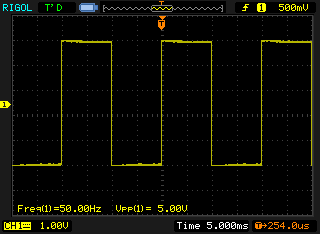
\includegraphics[width=0.48\textwidth]{Imagenes/ActividadPractica/MedicionDeTensionEficaz/Exp1_OndaCuadrada.png}}
        \caption{Señal cuadrada a medir.}
        \label{fig:SeñalCuadrada}
      \end{figure}

      \begin{figure}[H]
        \centering
        \begin{subfigure}[ht]{0.48\textwidth}
          \frame{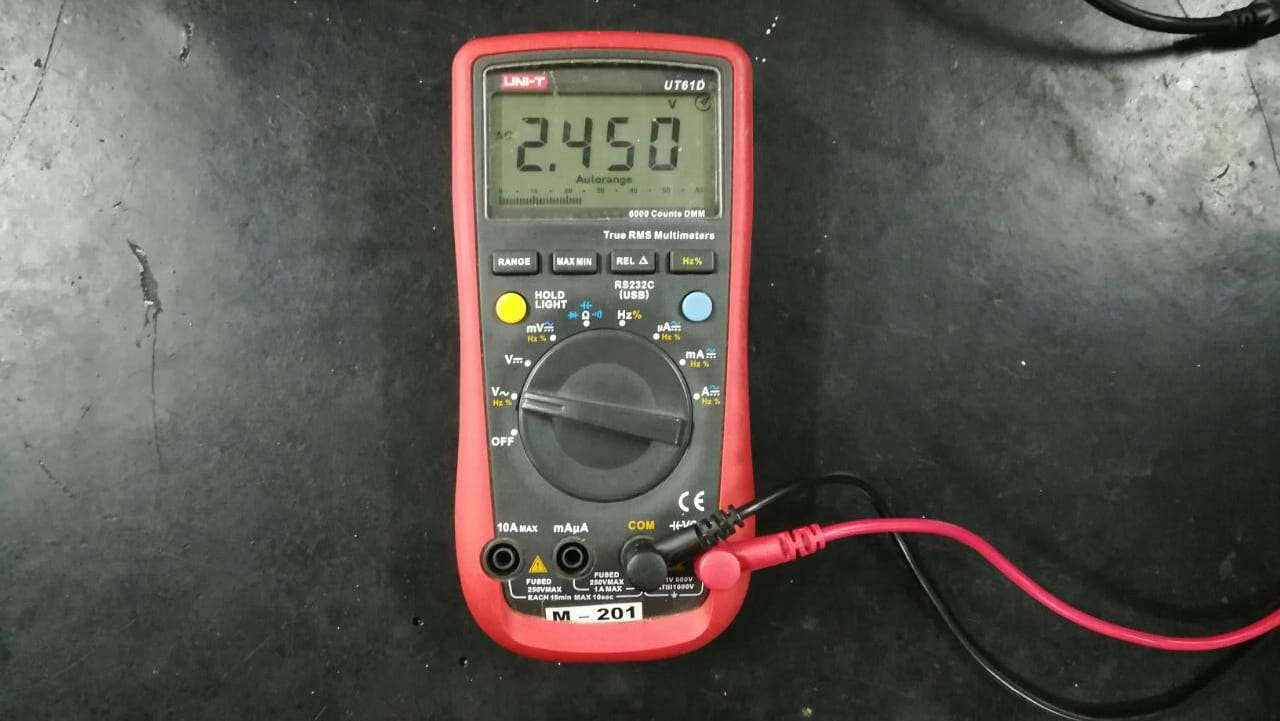
\includegraphics[width=\textwidth]{Imagenes/ActividadPractica/MedicionDeTensionEficaz/Exp1_Vrms_Cuadrada.jpeg}}
          \caption{Medición $V_{RMS}$.}
          \label{fig:MedicionVrmsCuadrada}
        \end{subfigure}
        \hfill 
        \begin{subfigure}[ht]{0.48\textwidth}
          \frame{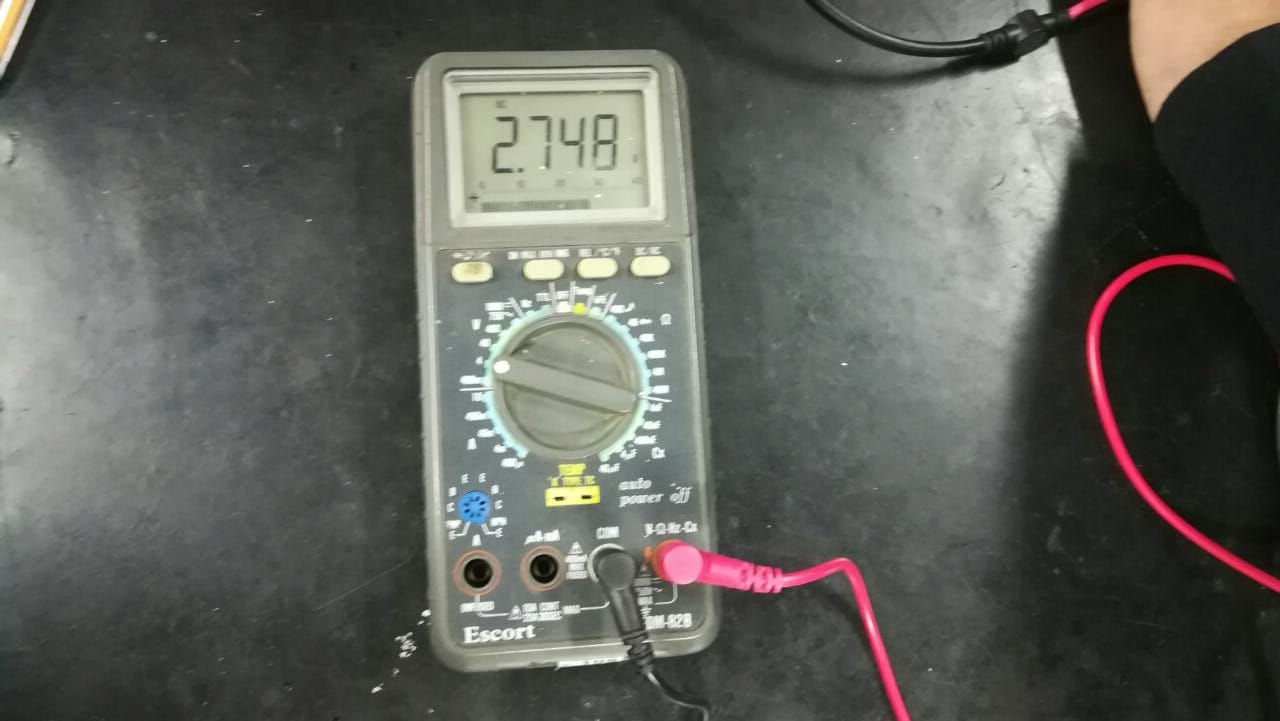
\includegraphics[width=\textwidth]{Imagenes/ActividadPractica/MedicionDeTensionEficaz/Exp1_Vmed_Cuadrada.jpeg}}
          \caption{Medición $V_{|med|}$.}
          \label{fig:MedicionVmedCuadrada}
        \end{subfigure}
        \caption{Mediciones de la señal cuadrada.}
         \label{fig:MedicionSeñalCuadrada}
      \end{figure}


      Luego, la cota de corrección para el multímetro de respuesta al valor medio del módulo es

      \begin{align*}
        e_{cuad} [\%] = \dfrac{V_{RMS} - V_{|med|}}{V_{|med|}} \cdot 100
               = \dfrac{2,450~V - 2,748~V}{2,748V} \cdot 100
               \hspace{20pt} \therefore \hspace{10pt} \Aboxed{e_{cuad} = -10,84\%}~.
      \end{align*}


    \subsubsection{En una onda triangular}
      En la Figura~\ref{fig:SeñalTriangular} se puede observar la señal triangular seteada.
      Luego, en la Figura~\ref{fig:MedicionSeñalTriangular} se observa la medición de tensión
      con ambos multímetros.

      \begin{figure}[H]
        \centering
        \frame{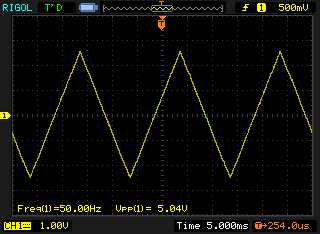
\includegraphics[width=0.45\textwidth]{Imagenes/ActividadPractica/MedicionDeTensionEficaz/Exp1_OndaTriangular.png}}
        \caption{Señal triangular a medir.}
        \label{fig:SeñalTriangular}
      \end{figure}

      \begin{figure}[H]
        \centering
        \begin{subfigure}[ht]{0.48\textwidth}
          \frame{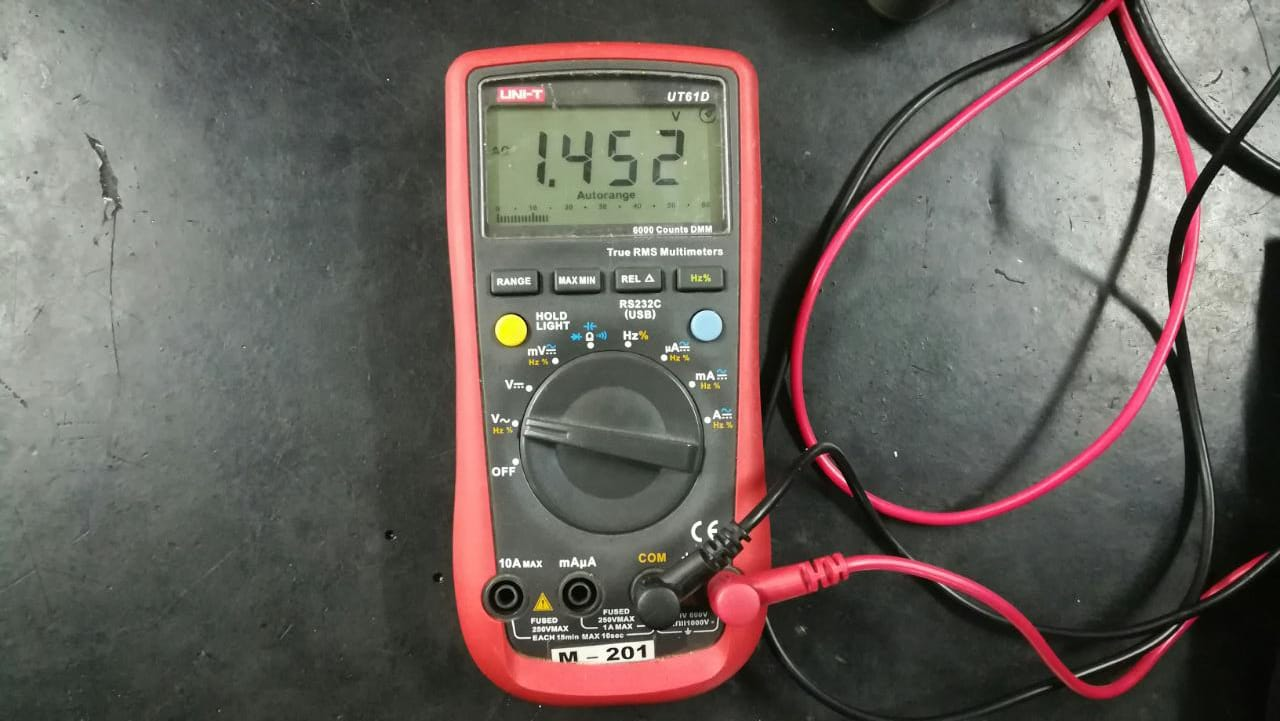
\includegraphics[width=\textwidth]{Imagenes/ActividadPractica/MedicionDeTensionEficaz/Exp1_Vrms_Triangular.jpeg}}
          \caption{Medición $V_{RMS}$.}
          \label{fig:MedicionVrmsTriangular}
        \end{subfigure}
        \hfill 
        \begin{subfigure}[ht]{0.48\textwidth}
          \frame{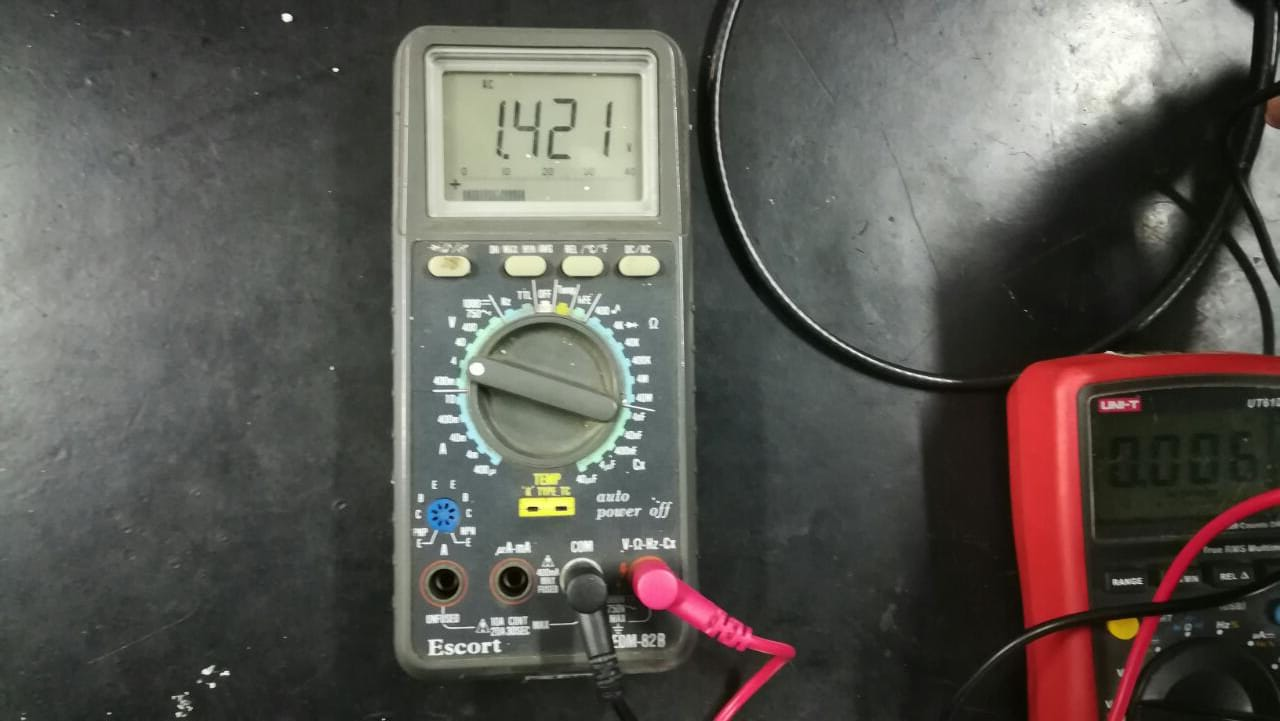
\includegraphics[width=\textwidth]{Imagenes/ActividadPractica/MedicionDeTensionEficaz/Exp1_Vmed_Triangular.jpeg}}
          \caption{Medición $V_{|med|}$.}
          \label{fig:MedicionVmedTriangular}
        \end{subfigure}
        \caption{Mediciones de la señal triangular.}
         \label{fig:MedicionSeñalTriangular}
      \end{figure}

      Luego, la cota de corrección para el multímetro de respuesta al 
      valor medio del módulo es

      \begin{align*}
        e_{tri} [\%] = \dfrac{V_{RMS} - V_{|med|}}{V_{|med|}} \cdot 100
               = \dfrac{1,452~V - 1,421~V}{1,421~V} \cdot 100
               \hspace{20pt} \therefore \hspace{20pt} \Aboxed{e_{tri}= +2,18\%}~.
      \end{align*}

    Los resultados de este experimento se encuentran consignados en la
    Tabla~\ref{tab:MedicionesOndasCuadYTrian}.
  
    \begin{table}[H] \centering
      \begin{tabular}{|c|c|c|c|} \hline
        \textbf{Señal}     & \textbf{Lectura RMS [V]}  & \textbf{Lectura |med| [V]} & \textbf{e [\%]} \\ \hline
      $\mathbf{Cuadrada~(50~Hz - 5~V_{pp})}$    & 2,450     & 2,748         &  -10,84        \\ \hline
      $\mathbf{Triangular~(50~Hz - 5~V_{pp})}$  & 1,452      & 1,421        &  +2,18         \\ \hline
      \end{tabular}
      \caption{Tabla de mediciones y cotas de corrección.}
      \label{tab:MedicionesOndasCuadYTrian}
    \end{table}

      \subsection{Medición de la tensión eficaz de una onda proveniente de un circuito de control de ángulo de conducción}

      \subsection{Medición de factor de potencia en un circuito con control de ángulo de conducción}

Para el siguiente experimento se emplea el mismo circuito de la sección anterior. 
Ésta vez se conecta al medidor digital para medir 
el factor de potencia.

\begin{figure}[H]
  \centering
  \frame{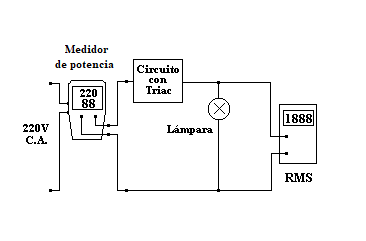
\includegraphics[width=0.5 \textwidth]{Imagenes/ActividadPractica/MedicionDeFactorDePotenciaConCircuitoTriac/Circuito_Medicion_FP_TriacDiac.png}}
  \caption{Circuito de medición de factor de potencia.}
  \label{fig:CircuitoMideFDP}
\end{figure}

Una vez realizada la conexión, se debe variar el potenciómetro del circuito 
de control de disparo, hasta lograr que la tensión eficaz de 
salida sea de 110~V.

\begin{figure}[H]
  \centering
  \frame{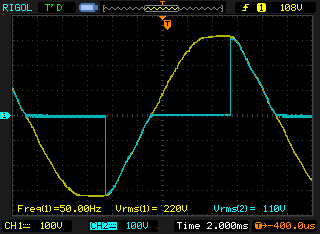
\includegraphics[width=0.5 \textwidth]{Imagenes/ActividadPractica/MedicionDeFactorDePotenciaConCircuitoTriac/Exp3_AnguloDisparoPara110Vrms.png}}
  \caption{Forma de onda para una tensión eficaz de 110[V].}
  \label{fig:SeñalExp3}
\end{figure}

 En éste punto se mide el factor de potencia inicial, 
 cuyo valor es de 0,47.

 \begin{figure}[H]
  \centering
  \frame{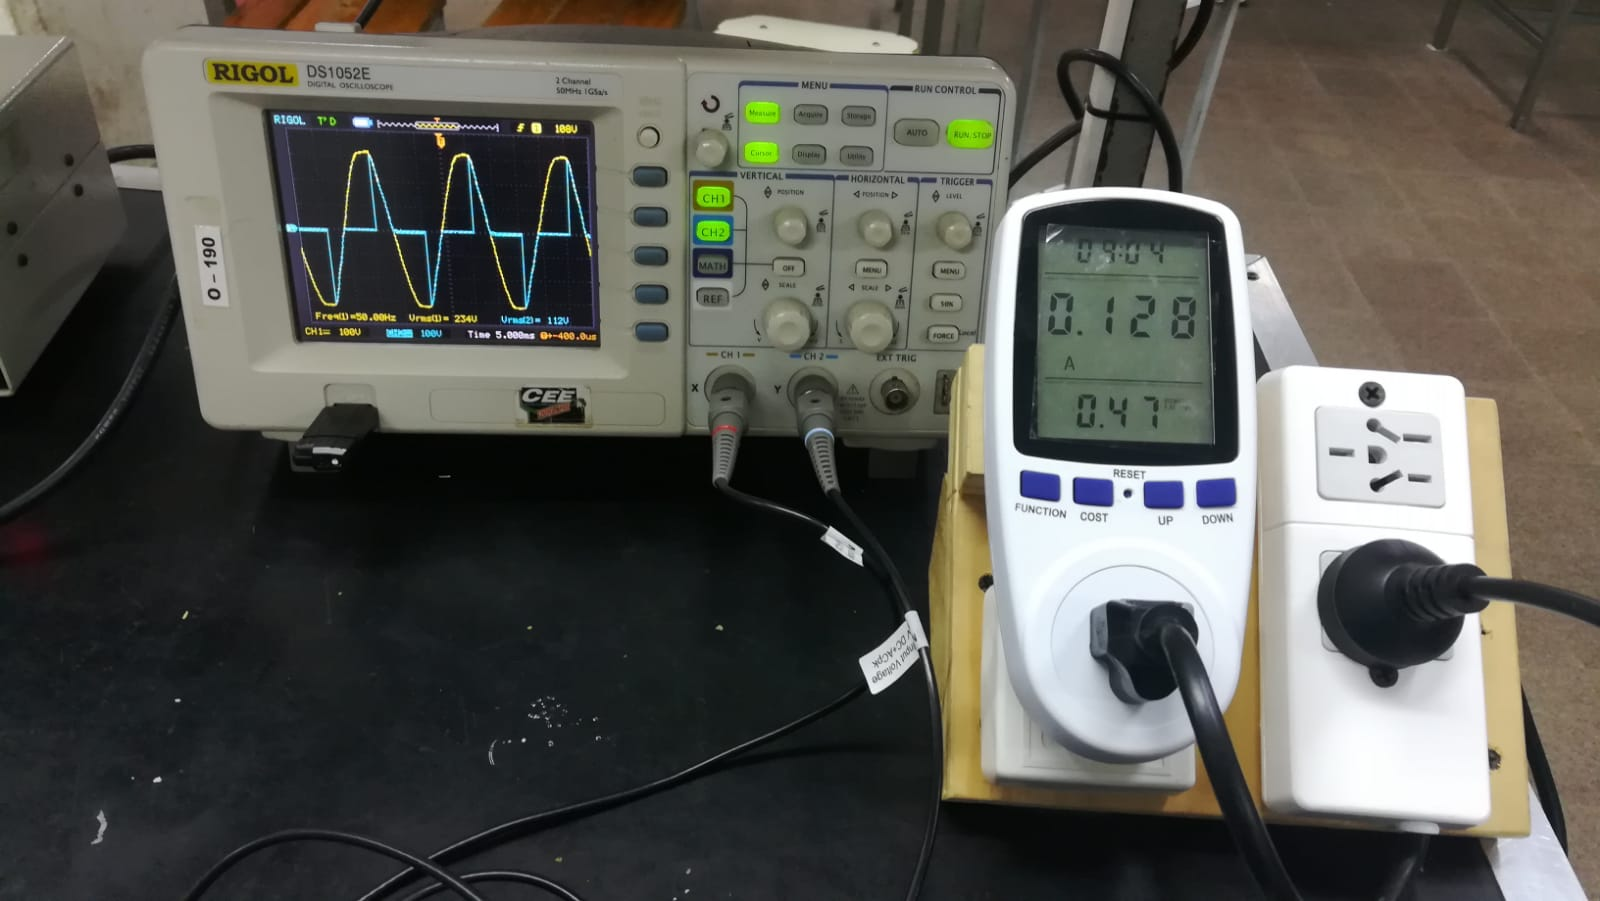
\includegraphics[width=0.5 \textwidth]{Imagenes/ActividadPractica/MedicionDeFactorDePotenciaConCircuitoTriac/Exp3_FDPcon110Vrms.jpeg}}
  \caption{Factor de potencia inicial.}
  \label{fig:FDPExp3}
\end{figure}

Al conectar el capacitor de corrección, se observa que el factor 
de potencia aumenta a 0,55, como muestra la Figura~\ref{fig:FDPCorregidoExp3}. 
Ésto indica que la carga total del circuito en conjunto, se comporta de manera inductiva.

 \begin{figure}[H]
  \centering
  \frame{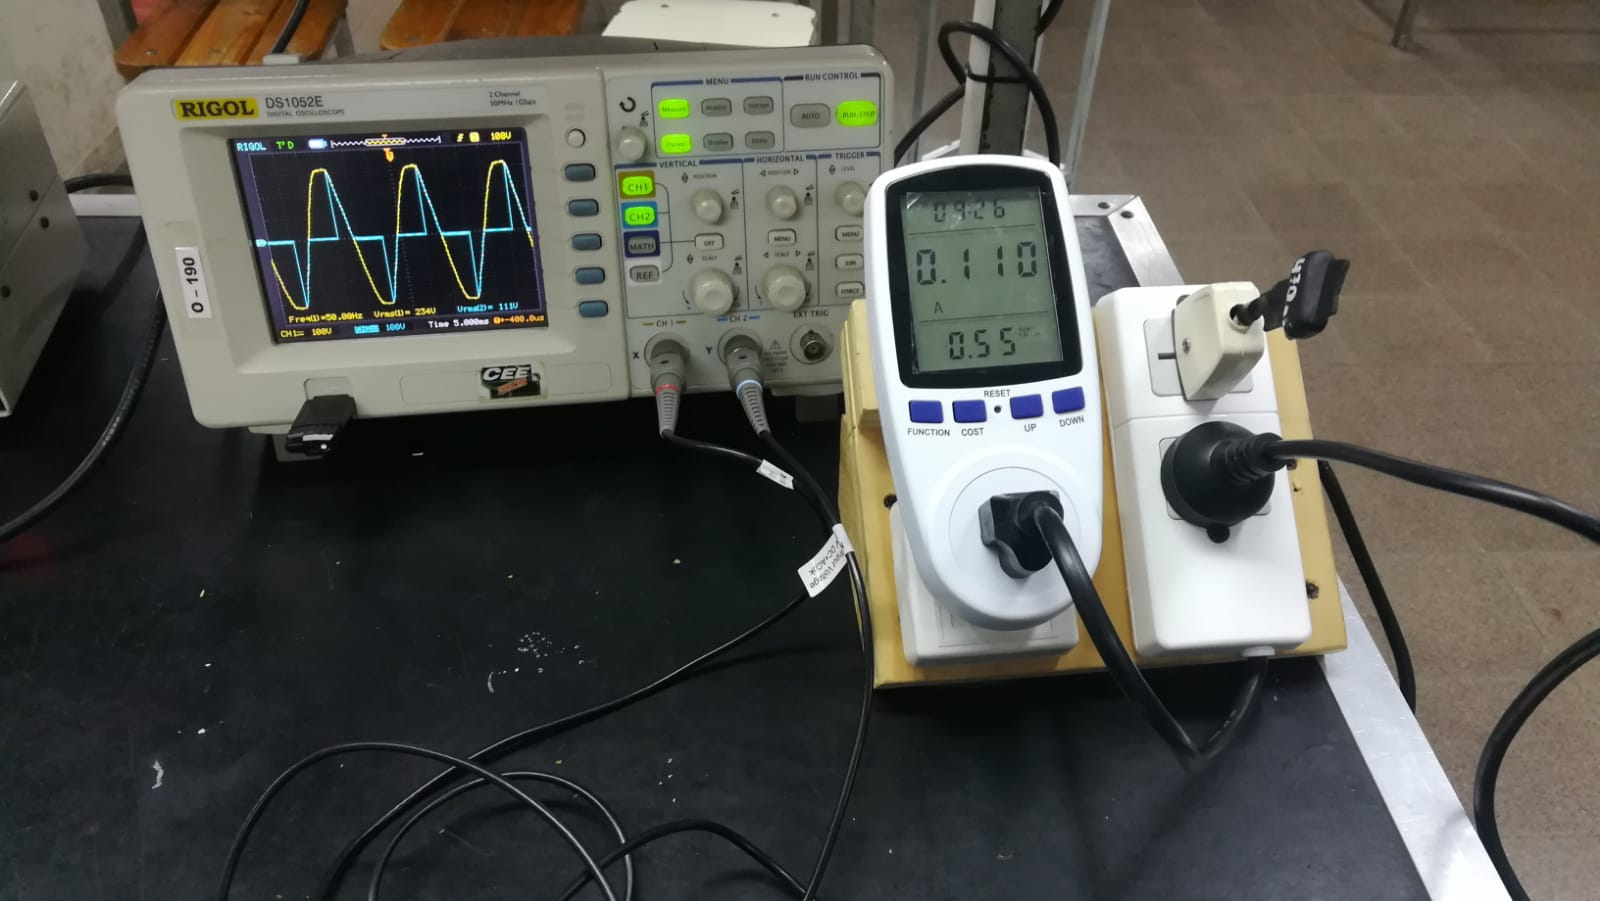
\includegraphics[width=0.5 \textwidth]{Imagenes/ActividadPractica/MedicionDeFactorDePotenciaConCircuitoTriac/Exp3_FDPConCapacitor.jpeg}}
  \caption{Factor de potencia corregido.}
  \label{fig:FDPCorregidoExp3}
\end{figure}


    \pagebreak
  \section{Conclusiones}
    En relación con el primer experimento realizado en este trabajo
    práctico, se procede a obtener de forma analítica los valores
    de las cotas de corrección de las mediciones realizadas con
    el multímetro con respuesta al valor medio del módulo de la 
    tensión.
    
    Se sabe que los multímetros de respuesta al valor medio del
    módulo, realizan una corrección mediante una cota para obtener 
    el valor eficaz de la medición. Para obtener dicha cota, se 
    hace uso de los siguientes valores representativos de una 
    \textbf{señal senoidal}

    \vspace{-5pt}
    $$ V_{RMS_{\sin}} = \dfrac{V_{\max}}{\sqrt{2}} \hspace{20pt} ; 
    \hspace{20pt} V_{|med|_{\sin}} = \dfrac{2\, V_{\max}}{\pi}~. $$

    \noindent Luego, el factor de forma se obtiene
    relacionando las expresiones anteriores
    
    \vspace{-5pt}
     $$ k = \dfrac{V_{RMS_{\sin}}}{V_{|med|_{\sin}}} 
        = \dfrac{\dfrac{V_{\max}}{\sqrt{2}}}{\dfrac{2\, V_{\max}}{\pi}}
        \hspace{20pt} \Longrightarrow \hspace{20pt} k = 1,1107~.$$

    El valor antes encontrado, es el que permite saber que el multímetro
    de respuesta al valor medio del módulo muestra en el display el 
    resultado de $ V_{lectura} = 1,1107 \cdot V_{|med|}~. $

    Teniendo en cuenta lo mencionado anteriormente, y que para una señal cuadrada
    su valor eficaz y valor medio de módulo se expresan mediante

    \vspace{-5pt}
    $$ V_{RMS_{cuad}} = V_{\max} \hspace{20pt} ; \hspace{20pt} V_{|med|_{cuad}} = V_{\max}~, $$

    \noindent entonces, el error porcentual para la medición de 
    la señal cuadrada es

    \vspace{-5pt}
    $$ e_{cuad} [\%] = \dfrac{k \cdot V_{|med|_{cuad}} -  V_{RMS_{cuad}}}{V_{RMS_{cuad}}} \cdot 100
              = \dfrac{1,1107\, V_{\max} - V_{\max}}{V_{\max}} \cdot 100 $$
              $$  \therefore \hspace{20pt} \boxed{e_{cuad}[\%] = +11,07\%}~.
    $$

    Siguiendo la misma línea, para una señal triangular sus valor eficaz y valor
    medio de módulo se expresan mediante

    \vspace{-5pt}
$$ V_{RMS_{tri}} = \dfrac{V_{\max}}{\sqrt{3}} \hspace{20pt} ; \hspace{20pt} V_{|med|_{tri}} = \dfrac{V_{\max}}{2}~, $$

    \noindent entonces, el error porcentual para la medición de 
    la señal triangular es

    \vspace{-5pt}
    $$ e_{tri} [\%] = \dfrac{k\cdot V_{|med|_{tri}} - V_{RMS_{tri}}}{V_{RMS_{tri}}} \cdot 100
    = \dfrac{ 1,1107\, \dfrac{V_{\max}}{2} - \dfrac{V_{\max}}{\sqrt{3}} }{\dfrac{V_{\max}}{\sqrt{3}}} \cdot 100 $$
              $$  \therefore \hspace{20pt} \boxed{e_{tri}[\%] = -3,81\%}~.
    $$

    En la Tabla~\ref{tab:ComparacionCotas}, se puede observar la comparación entre valores
    prácticos y teóricos de las mediciones realizadas con el multímetro de respuesta al 
    valor medio del módulo. Los valores presentan diferencias entre sí, en especial
    en el caso de la señal triangular. Esto se
    puede fundamentar en base a que, el factor de forma de la señal triangular indica que el valor eficaz
    difiere un 15\% aproximadamente del valor medio del módulo, siendo que el instrumento está
    diseñado para medir éste último. Por otro lado, en la señal cuadrada ambos valores
    son iguales, lo que justifica que la diferencia de error sea menor.

    \begin{table}[H] \centering
      \begin{tabular}{|c|c|c|c|} \hline
        \textbf{Señal}       & \textbf{Error práctico [\%]}  & \textbf{Error teórico [\%]} & \textbf{Factor de forma} \\ \hline
        Cuadrada    & +12,16               & +11,07              &  1,000              \\ \hline
        Triangular  & -2,13                & -3,81              &  1,1547         \\ \hline
      \end{tabular}
      \caption{Tabla de comparación de cotas.}
      \label{tab:ComparacionCotas}
    \end{table}

En relación con el tercer experimento, se observó que el comportamiento del 
circuito (según la lectura del factor de potencia del dispositivo empleado), 
es de tipo inductivo, ya que al conectar el capacitor, el factor de potencia 
mejoró.

Para comenzar análisis, se supone el método de medición de cruces 
por cero de la señal de tensión y corriente, que consiste en medir el retardo entre 
ambas señales.
Al variar el potenciómetro del circuito de control de ángulo de disparo, se modifica la constante 
de tiempo $\tau$ de carga y descarga del capacitor, lo que provoca un retardo en el disparo de la 
señal de la corriente de entrada, como puede observarse en la Figura \ref{fig:SeñalExp3}, ya que 
se modifica el instante en que conduce el diac. Esto provoca que el medidor detecte un falso desfasaje. 



%  De ésta manera, al modificar el circuito conectando 
% un segundo capacitor a la salida, dicha tensión del capacitor de entrada se ve alterada y, por 
% lo tanto, el ángulo de disparo también. Entonces, puede decirse que la mejora del factor 
% de potencia, marcada por el medidor se debe a que al conectar el capacitor, el cruce por 
% cero se mueve junto con el ángulo de disparo en forma de adelanto respecto al punto original.

% Para realizar el segundo análisis a partir de la topología del circuito, se debe 
% tomar un punto de referencia. Para ello se supone las condiciones 
% inciales de la siguiente manera: El TRIAC no está en región de conducción, por 
% lo tanto el DIAC tampoco, pudiendo representarlos como 
% un circuito abierto en el esquema de la Figura \ref{fig:CircuitoTriacDiac}. La 
% segunda condición, es que el capacitor inicia totalmente descargado.

% Bajo las suposiciones anteriores, el circuito resultante será el que se enseña 
% en la Figura \ref{fig:ConclusionRCTriac}.

% \begin{figure}[H]
%   \centering
%   \frame{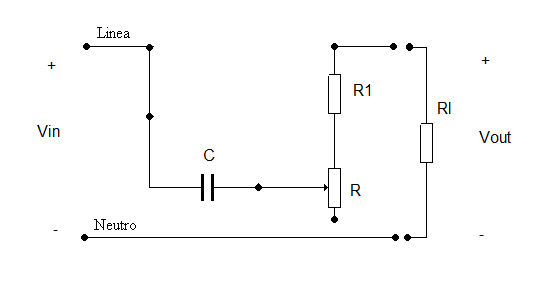
\includegraphics[width=0.8\textwidth]{Imagenes/Conclusiones/Exp3_Circuito en condicion inicial.png}}
%   \caption{Situación inicial del circuito con TRIAC.}
%   \label{fig:ConclusionRCTriac}
% \end{figure}

% Como puede observarse, se trata de un circuito adelantador de fase, cuya 
% respuesta en frecuencia, puede demostrarse que se comporta como un circuito RL 
% serie.

% La explicación de que el dispositivo utilizado para medir el factor de potencia, 
% tome al circuito como de naturaleza inductiva, se debe al adelanto de fase de la 
% señal de tensión de salida, respecto de la de entrada.

% Una vez que la tensión en el capacitor alcanza los 30[V] , el DIAC entra en región 
% de conducción reduciendo su resistencia dinámica al mínimo, polarizando a su vez el 
% TRIAC, y cerrando el ciclo de carga-descarga del capacitor. En éste punto, el sistema 
% posee un comportamiento resistivo puro.

% Como la condición impuesta en un principio, se mantiene 
% al menos la mitad del ciclo de onda, se podría decir que tendrá comportamiento mayormente 
% reactivo, de ésta manera, el dispositivo de medición determina que el circuito tiene 
% características inductivas.







  
\end{document}
